%!TEX root = bare_conf.tex

\section{Testgetriebene Entwicklung} \label{sec:tdd}

Die testgetriebene Entwicklung (TDD) ist eine der zentralen Praktiken des XPs, kann aber auch unabhängig davon angewendet werden. Die Methode setzt auf kurze Iterationen, in denen sowohl die Software als auch die Software-Architektur schrittweise entsteht. Anders als der Name vermuten lässt, ist TDD keine Teststrategie \cite{Janzen2005Test-drivenDirection}.

Nichtsdestotrotz beginnt jede Iteration mit dem Schreiben eines Tests. Anschließend wird genauso viel Code geschrieben, wie der Test für eine erfolgreiche Prüfung benötigt. Sobald der Test mit einem positiven Ergebnis durchgelaufen ist, kann, falls nötig, die bestehende Codebasis einem \textit{Refactoring} unterzogen werden \cite{Janzen2005Test-drivenDirection}.

Während des Refactoring wird die interne Struktur von existierenden und funktionierenden Programmcodes verbessert. Ziel ist es, den Code verständlicher zu machen, ohne neue Funktionalität hinzuzufügen \cite{Link2005SoftwaretestsEntwicklung}.

Etwas formaler kann die testgetriebene Entwicklung anhand von zwei Regeln beschrieben werden \cite{Beck2003TestExample}:
\begin{itemize}
\item Es soll nur neuer Code geschrieben werden, wenn ein Test fehlschlägt.
\item Redundanzen sollen eliminiert werden.
\end{itemize}
Diese beiden Regeln geben die Reihenfolge der Arbeitsschritte bei der Entwicklung vor \cite{Beck2003TestExample}:
\begin{enumerate}
\item Schreibe einen Test der kompiliert, aber fehlschlägt (Red).
\item Schreibe gerade so viel Code, dass der Test läuft (Green).
\item Überarbeite den Code, so dass keine Redundanzen mehr enthalten sind (Refactor).
\end{enumerate}
Insgesamt kann der Ablauf von der TDD mit dem kurzen Mantra „Red/Green/Refactor“\footnote{Fehlgeschlagene Tests werden in der Praxis oft durch die Farbe Rot und erfolgreiche Tests durch die Farbe Grün signalisiert.} beschrieben werden \cite{Beck2003TestExample}. In Abbildung \ref{fig:TDDvsTLD} sind die Unterschiede von TDD und TLD in Form zweier Aktivitätsdiagramme dargestellt.

\begin{figure*}[tbh]
\centering
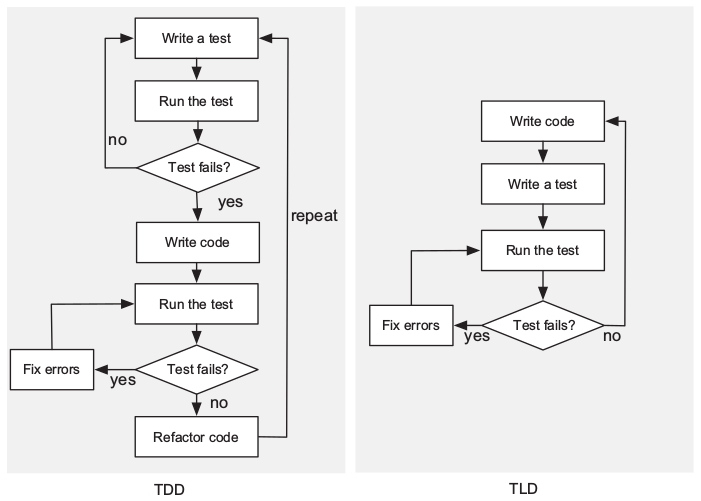
\includegraphics[scale=0.6]{tdd_vs_tld}
\caption{TDD vs. TLD, aus \cite{Munir2014ConsideringReview}}
\label{fig:TDDvsTLD}
\end{figure*}

Im Folgenden sind Vor- und Nachteile von der TDD aufgelistet, die häufig in der Literatur genannt werden. Im Anschluss sind positive und negative Auswirkung von der TDD beschrieben, die in Studien ermittelt wurden.

\subsection{Vorteile der testgetriebenen Entwicklung}  \label{sec:tddVorteile}
Nachfolgend sind Vorteile von der TDD beschrieben.

\subsubsection{Testabdeckung/Flexibilität} In der TDD soll neue Funktionalität nur dann hinzugefügt werden, wenn zuvor der entsprechende Test geschrieben wurde. Dadurch wird sichergestellt, dass nahezu der gesamte Code der Anwendung getestet ist. Die so erreichte hohe Testabdeckung, ermöglicht es, den gesamten Programmcode auf Fehler zu prüfen. Dies hilft dem Entwickler festzustellen, ob beispielsweise eine vorgenommene Änderung im Code, an einer anderen Stelle versehentlich einem Fehler in Programmablauf hervorruft. Der Code bleibt durch die hohe Testabdeckung flexibler.\cite{Martin2007ProfessionalismDevelopment, Janzen2005Test-drivenDirection}.

Die hohe Testabdeckung erlaubt es außerdem, eine Aussage über die Funktionsfähigkeit der Anwendung zu machen. Dies ist sowohl für die Planung als auch die Durchführung einer Softwareintegration wichtig \cite{Link2005SoftwaretestsEntwicklung}.

\subsubsection{Programmdesign} Eine Klasse lässt sich einfacher Testen, wenn sie keine oder wenig Abhängigkeit zu einer anderen Klasse besitzt. Durch die TDD werden die Entwickler ständig angehalten, auf eine lose Kopplung bei den Entwurf von Klassen zu achten \cite{Martin2007ProfessionalismDevelopment, Link2005SoftwaretestsEntwicklung,Yahya2015TheDevelopment}.

Allerdings heißt es auch in Martin \cite[S. 35]{Martin2007ProfessionalismDevelopment}: „Good designs aren’t free, and TDD doesn’t guarantee good designs. However, TDD provides powerful impetus to decouple, forcing developers to think through their designs in ways that they otherwise might not.“ Die TDD kann den Entwickler also nur dazu bringen auf das Design zu achten, aber dies muss nicht unweigerlich zu einen guten Design führen.

\subsubsection{Motivation} Bei der traditionellen Entwicklung, wird mit der Implementierung der Funktionalität begonnen und im Anschluss sollen die Tests geschrieben werden, um die Funktionalität zu prüfen. Häufig fehlt dem Entwickler jedoch die Motivation nach der Implementierung noch Tests zu schreiben. Er ist sich sicher, dass seine Implementierung fehlerfrei ist. Es ist für ihn dann oft interessanter, mit der Implementierung des nächsten Features zu beginnen. Die ohnehin geringe Motivation Tests zu schreiben, kann zusätzlich noch negativ beeinflusst werden, wenn die Abhängigkeiten zwischen den erstellten Klassen sehr groß sind, da dies das Schreiben von Tests erschwert. Beim TDD werden diese Probleme umgangen, da die Entwicklung mit dem Schreiben des Tests startet \cite{Link2005SoftwaretestsEntwicklung}.

In Shull \cite[S. 17]{Shull2010WhatDevelopment} heißt es, dass TDD hilft Schludrigkeiten zu verhindern und Disziplin beim Programmieren fördert: „He [Grigori] described working with a young, energetic programmer whose work unfortunately included many mistakes. Following TDD rigorously helped the programmer become more intentional in his work, thinking through the functionality he wanted to add. TDD doesn’t just require skill and discipline; it also helps develop them.“

\subsubsection{Dokumentation} Ein der Teil der Dokumentation des Codes erfolgt in Form von Tests. Die Tests geben Auskunft über die normale Verwendung von Klassen und deren Umgang mit Ausnahmen. Außerdem können die Tests als Kommunikationsgrundlage für den Austausch mit anderen Entwicklern dienen \cite{Link2005SoftwaretestsEntwicklung, Martin2007ProfessionalismDevelopment}.

Diese Dokumentation in Form von (Test-)Code wird von jedem Entwickler verstanden. Und dass die Tests bzw. die Dokumentation immer auf dem aktuellen Stand sind, ist durch das Vorgehen der TDD festgelegt. Jedoch muss für eine gute Lesbarkeit der Tests, bei deren Erstellung mit entsprechender Sorgfalt vorgegangen werden \cite{Martin2007ProfessionalismDevelopment}.

\subsubsection{Feedback/Unsicherheiten nehmen} TDD kann dabei helfen mit Unsicherheiten bei der Entwicklung umzugehen, die einen begegnet, wenn man auf ein schwer zu lösendes Problem trifft. Wenn Unsicherheiten einen zaghaft, weniger Kommunikativ und ängstlich gegenüber Fehlern machen, soll TDD den Entwickler, durch das kleinschrittige Vorgehen, unterstützen schnell zu lernen, klarer zu kommunizieren und konkretes Feedback zu finden \cite{Beck2003TestExample}.

Dies wird auf verschiedene Weise erreicht. Durch die vielen kurzen Iterationen erhält der Entwickler häufig Feedback. Eine fremde Schnittstelle kann mit der Hilfe von Tests schrittweise kennengelernt werden. Schwer zu lösende Probleme können in kleinere, einfacher zu lösende Probleme aufgeteilt und schrittweise bearbeitet werden. Dabei wird durch die Tests, für jeden Schritt ein Maß an Korrektheit sichergestellt, welches bei der Entwicklung ohne Tests fehlen würde. Durch die vielen Tests, erhält man ein sehr granulares Feedback, so dass weniger Zeit im Debugger verbracht werden muss, um die Ursache eines Fehlers zu finden  \cite{Beck2003TestExample, Link2005SoftwaretestsEntwicklung, Martin2007ProfessionalismDevelopment}.

\subsection{Nachteile der testgetriebenen Entwicklung} \label{sec:tddNachteile}
Kollanus \cite{Kollanus2011CriticalDevelopment} listet einige potentielle Probleme von TDD auf.

\subsubsection{Testabdeckung/Flexibilität} Typischerweise ist das Verhältnis zwischen Test- und Produktionscode eins zu eins. In großen Projekten kann eine große Menge von Testfällen zu verschiedenen Problemen führen. Zum einen kann die Entwicklungszeit durch die vielen Tests stark verzögert werden, wenn das Ausführen aller Tests beispielsweise mehrere Minuten in Anspruch nimmt. In solchen Fällen, kann nur noch eine Untermenge der Tests nach jeder Iteration durchlaufen werden. Zum anderen benötigt das Refactoring mehr Aufwand, wenn viele Testfällen von den Änderungen betroffen sind, und angepasst werden müssen \cite{Kollanus2011CriticalDevelopment}.

\subsubsection{Programmdesign} Das Fehlen einer vorab durchgeführten, detaillierten Designphase kann zu einem mangelhaften Design der Anwendung führen. Was wiederum ein umfangreiches Refacotring zur Folge haben kann \cite{Kollanus2011CriticalDevelopment}.

\subsubsection{Motivation} Es ist schwer die TDD im Unternehmen einzuführen, da es nicht leicht zu lernen ist und mehr Aufwand und Zeit benötig als zunächst von den Entwicklern erwartet wird. Außerdem ist die Grundeinstellung gegenüber TDD bei einigen negativ. Zum einen wird die Produktivität des Verfahrens hinterfragt. Zum anderen möchten einige Entwickler ungern ihre Art zu programmieren ändern. Und selbst, wenn die Entwickler von möglichen Vorteilen überzeugt sind, fehlt es an Motivation die TDD praktisch anzuwenden, da der Aufwand für den Einzelnen zu hoch ist \cite{Kollanus2011CriticalDevelopment}.

\subsubsection{Erforderliches Fähigkeitslevel} Obwohl der Ablauf der testgetriebenen Entwicklung überschaubar ist (Red/Green/Refactore), gibt es einige Probleme, auf die Anfänger zu Beginn schnell stoßen. Der Entwickler benötigt ein Big-Picture des Programms, um Tests schreiben zu können. Erfahrene Entwickler können das Design im Kopf entwerfen, und daher funktioniert die TDD für sie. Auf Anfänger trifft dies jedoch nicht zu. Neben dem Problem, zu bestimmen \textit{was} getestet werden soll, bereitet zusätzlich auch das \textit{wie} ein Tests geschrieben wird, einem Anfänger Probleme. Direkt beim Schreiben des ersten Tests, stellt sich beispielsweise die Frage, wie groß ein Test bzw. eine Iteration sein sollte. Insgesamt erfordert es viel Übung, bis ein Entwickler fähig ist, gute Testfälle zu schreiben. Anfänger können damit schnell überfordert sein \cite{Kollanus2011CriticalDevelopment, Beck2003TestExample}.

Die Umfrage von Aniche und Gerosa \cite{Aniche2010MostDevelopers} zeigt ebenfalls Schwierigkeiten, die die Entwickler mit der testgetriebenen Entwicklung haben. Sie befragten 218 Entwickler nach den Fehlern, die ihnen bei dem TDD-Prozess \textit{häufig oder immer} unterlaufen:
\begin{itemize}
  \item 26.61\% schreiben zu komplexe Testszenarien.
  \item 23.85\% führen ein Refactoring eines anderen Codeteils durch, anstatt den Teil zu korrigieren, der einen Tests fehlschlagen lässt.
  \item 19.72\% vergessen den Refactoring-Schritt durchzuführen.
  \item 15.14\% halten sich nicht an die Empfehlung, mit dem Schreiben des einfachsten Tests zu beginnen.
  \item 14.22\% vergessen zu prüfen, ob der gerade geschriebene Test tatsächlich fehlschlägt.
  \item 11.01\% verwenden schlechte Testname.
  \item 11,01\% implementieren nicht nur den nötigsten Code, damit der Test erfolgreich ist.
  \item 8.72\% vergessen den Testcode einem Refactoring zu unterziehen.
  \item 5.96\% vergessen am Ende einer Iteration alle Tests ausführen.
\end{itemize}

%Experten halten sich mehr an die Regeln des TDD als Anfänger. Die Zyklen/Arbeitsschritte sind kürzer ein die Länge einheitlicher als bei Anfängern. Dennoch konnten einige Anfänger schon nach einer Woche intensives Training ähnliche Werte erzielen, wie die Experten. Die Anzahl der Zyklen ist im Durchschnitt gleich, unter den Anfängern variiert diese Zahl jedoch stärker. Beide Gruppen haben gleich viele Änderungen an Codezeilen vorgenommen.Experte führen schneller Änderungen am Anwendungscode durch als die Anfänger. Die Anfänger sind bei der Änderung von Testcode schneller. Die Experten sind bei der Entwicklung signifikant schneller. Allerdings ist die Codeabdeckung der Experten-Testfälle größer. Größe der Programme ist unterschiedlich, aber nicht signifikant.
%Keine Hinweise, inwiefern die IDE unterstützung für TDD von den IDEs genutzt wurde \cite{Muller2007TheProcess}.

%\cite{Rafique2013TheMeta-Analysis} Entwicklererfahrung hat Einfluss auf TDD.

\subsubsection{Anwendbarkeit} Ungeachtet der Erfahrung des Entwicklers, kann es je nach Kontext sehr schwer sein, Tests zu schreiben. Dies gilt zum Beispiel für das Schreiben von Tests für Benutzeroberflächen. Ein weiteres Beispiel sind eingebettete Systeme, da es unter Umständen unmöglich sein kann, die Tests auf der Zielhardware auszuführen. In manchen Fällen ist die Anwendbarkeit der TDD abhängig von den zur Verfügungen stehenden Entwicklungswerkzeugen. Ohne die passenden Werkzeuge bzw. Werkzeugunterstützung, kann die TDD schnell zu Zeitaufwändig werden \cite{Kollanus2011CriticalDevelopment}.

\subsubsection{Positives Test-Bias} Bei der TDD werden vor allem positive Testfälle geschrieben, d.h. es wird getestet wie das System im Normalfall reagieren soll. Negative Testfälle, beispielsweise fehlerhafte Benutzereingaben, werden seltener überprüft. Jedoch werden durch negative Testfälle mehr defekte gefunden als durch positive Testfälle. Negative Testfälle sind daher für die Entwicklung wichtig, werden bei der TDD aber zu wenig beachtet \cite{Causevic2013EffectsExperiment}.

% Positive Test Bias: TDD ist keine Teststrategie

\subsection{Auswertung Studien} \label{sec:tddAuswertungStudien}

In diesem Abschnitt werden die Ergebnisse der gefundenen Studien aus Abschnitt \ref{sec:tddMethode} vorgestellt. Die Auswirkungen von der TDD werden in Experimenten, Befragungen, Fallstudien durch verschiedenen Metriken beschrieben. Munir et al. \cite{Munir2014ConsideringReview} listet acht Variablen auf, die in seinen untersuchten Studien häufig verwendet wurden: Produktivität, Aufwand/Zeit, Größe, externe Qualität, interne Codequaltät, Entwicklermeinung, Robustheit und  Konformität. Für jede Variable nennt er wiederum verschiedene Metriken. Nachfolgend werden die Ergebnisse zur Produktivität, externe Qualität und interne Codequalität näher betrachtet. Diese wurden von den meisten der betrachteten Studien verwendet.

\subsubsection{Produktivität} In der Studie \cite{Gupta2007AnDevelopment} von Gupta und Jalote wurden 22 Studenten gleichmäßig in zwei Gruppen eingeteilt. Eine Gruppe entwickelte testgetrieben, die andere traditionell. Die Gruppe die testgetrieben entwickelte, benötigte im Durchschnitt weniger Zeit zum Lösen von zwei vorgegebenen Programmieraufgabe. Der unterschied zwischen beiden Gruppen war jedoch nicht statistisch signifikant. Berechnet wurde die Produktivität mit der Formel \ref{eqn:TDDProduktivitaet}, wobei NCLOC für nicht auskommentierte Codezeilen steht und DE, die Zeit für die Entwicklung in Personenstunden beschreibt.

\begin{equation}
\label{eqn:TDDProduktivitaet}
Produktivitaet = \frac{NCLOC}{DE}
\end{equation}

Mülller und Hagner \cite{Muller2002ExperimentProgramming} teilte die 19 Teilnehmer seiner Studie ebenfalls in eine TDD-Gruppe und eine TLD-Gruppe ein, bestehend aus 10 bzw. 9 Studenten. Die Arbeit der Teilnehmer wurde in zwei Phasen eingeteilt. In der erste Phase wurde eine Anwendung implementiert. In der zweiten Phase führten die Studenten Akzeptanztest aus und behoben gegebenenfalls Fehler in ihrer Implementierung. Für die Evaluation der Produktivität wurden verschiedene Zeiten und Brüche verglichen. Dazu gehörte die Zeit, die für die die komplette Aufgabe benötigt wurde, die Zeit die für die Implementierungsphase benötigt wurde und das Verhältnis zwischen den beiden zuvor genannten Zeiten. Hinsichtlich der für die Aufgabe insgesamt benötigten Zeit, wurde kein Unterschied zwischen den beiden Gruppen festgestellt.

An der Studie von Causevic et al. \cite{Causevic2012TestExperiment} nahmen 14 Studenten teil. Sie wurden in zwei Gruppen eingeteilt. Die eine Gruppe nutzte die TDD, um eine vorgegebene Aufgabe zu lösen. Die andere Gruppe ging traditionell vor.  Die TDD-Gruppe war im Durchschnitt eine Stunde vor der TLD-Gruppe mit der Entwicklung fertig. Dies war jedoch nicht statistisch signifikant.

In der Studie von Fucci et al. \cite{Fucci2016AnApproach} entwickelten 21 Studenten einen Tag testgetrieben und einen Tag traditionell. Es wurden 40 Beobachtungen von 20 gültigen Teilnehmern analysiert. Dabei konnten keine Unterschiede hinsichtlich der Produktivität zwischen der TDD und der TLD festgestellt werden.

In zwei Studien neigten die Entwickler die testgetrieben entwickelten dazu, produktiver zu sein \cite{Gupta2007AnDevelopment,Causevic2012TestExperiment}. Drei Studien konnten keinen Unterschied in der Produktivität zwischen TDD und TLD feststellen \cite{Gupta2007AnDevelopment,Muller2002ExperimentProgramming,Fucci2016AnApproach}.  Werden jedoch nur die statistisch signifikanten Ergebnisse betrachtet, konnte weder die TDD noch die TLD als produktivere Praktik identifiziert werden.

\subsubsection{Externe Codequalität} An der Studie von Madeyski \cite{Madeyski2005PreliminaryQuality} nahmen 188 Studenten teil. Die Studenten wurden in vier Gruppen eingeteilt. Für diesen Abschnitt sind zwei Gruppen interessant. Die eine Gruppe entwickelte testgetrieben und bestand aus 34 Studenten. Die andere Gruppe entwickelte traditionell und bestand aus 32 Studenten. Der von der TDD-Gruppe geschriebene Code bestand weniger Akzeptanztests als der Code der TLD-Gruppe. Die externe Codequalität war statistisch signifikant geringer.

Auch in Gupta und Jalote  \cite{Gupta2007AnDevelopment} wurde die externe Codequalität durch die Anzahl erfolgreich durchlaufener Akzeptanztests ermittelt. Die Studienteilnehmer mussten zwei Programmieraufgaben lösen. Für die eine Programmieraufgabe war die externe Codequalität der TDD-Gruppe statistisch signifikant besser. Bei der anderen Aufgabe wurde kein statistisch signifikanter unterschied hinsichtlich der externe Codequalität zwischen den beiden Gruppen festgestellt. Für diese Aufgabe war die Anzahl der bestandenen Akzeptanztest bei der TLD-Gruppe höher, was eine bessere externe Codequalität vermuten lässt.

In Müller und Hagner \cite{Muller2002ExperimentProgramming} wurde die Anzahl der Fehler ebenfalls durch Akzeptanztest gemessen. Die externe Codequalität der TDD-Gruppe war nach der Implementierungsphase statistisch signifikant geringer. Nachdem die Studienteilnehmer Zeit hatten, die durch die Akzeptanztest aufgedeckten Fehler zu beheben, war die externe Codeqaulität der TDD-Gruppe ein wenig, jedoch nicht statistisch signifikant, besser als die der TLD-Gruppe.

Am Ende des Versuchs in Causevic et al. \cite{Causevic2012TestExperiment} wurde auf die Lösung jedes Teilnehmers, die Tests aller anderen Teilnehmer angewändet. Die fehlgeschlagenen Assertions dieser Tests wurden jeweils für jeden Teilnehmer gezählt und ausgewertet. Der Code der Teilnehmer die testgetrieben entwickelten, hatten im Durchschnitt weniger Defekte  als der Code der Teilnehmer die traditionell entwickelten. Der Unterschied war jedoch nicht statistisch signifikant.

Fucci et al. \cite{Fucci2016AnApproach} kam in seiner Sudie zu dem Ergebnisse, dass es kein Unterschied zwischen der TDD und der TLD hinsichtlich der externe Codequalität gibt. Die Codequalität wurde mit Hilfe von Akzeptanztests gemessen.

Für die externe Codequalität zeigt sich ein gemischtes Bild. In einer Studie gibt es keinen Unterschied zwischen TDD und TLD \cite{Fucci2016AnApproach}. Drei Studien erhalten keine statistisch signifikanten Ergebnisse. Davon tendieren in zwei der Studien die Teilnehmer, die TDD anwenden, zu besseren Ergebnissen \cite{Muller2002ExperimentProgramming, Causevic2012TestExperiment}. Die andere Studie kommt zu einem entgegengesetzten Resultat. In dieser liefert die TLD-Gruppe besseren Ergebnissen \cite{Gupta2007AnDevelopment}. Zwei Studien kommen zu statistisch signifikanten Ergebnissen. In \cite{Gupta2007AnDevelopment} schneidet TDD signifikant besser ab. Und in \cite{Madeyski2005PreliminaryQuality} ist wiederum TLD signifikant im Vorteil gegenüber TDD.

\subsubsection{Interne Codequalität} In der Studie von Madeyski \cite{Madeyski2010TheExperiment} wurden 19 Studenten in zwei Gruppen eingeteilt. Die TLD-Gruppe bestand aus zehn Studenten, die TDD-Gruppe aus neun. Zwischen den beiden Gruppen wurde kein statistisch signifikanter Unterschied hinsichtlich des Branch-Coverage gemessen. Die durchschnittliche Branch-Coverage  der TDD-Gruppe war, um 8\% Punkte höher.

Die Branch-Coverage wurde in Müller und Hagner \cite{Muller2002ExperimentProgramming} gemessen, nachdem die Aufgabe der Teilnehme vollständig abgeschlossen war. Die Ergebnisse der Messungen beider Gruppen waren ähnlich. Es konnte kein statistisch signifikanten Unterschied festgestellt werden.

In Causevic et al. \cite{Causevic2012TestExperiment} wurde die Code-Coverage der Teilnehmer untersucht. Im Durchschnitt war die Code-Covergage der TDL- und der TDD-Gruppe nahezu identisch.

Drei Studien haben die interne Codequalität untersucht. Zwei Studien konnten keinen Unterschied zwischen der TDD und der TLD feststellen \cite{Muller2002ExperimentProgramming,Causevic2012TestExperiment}. In \cite{Madeyski2010TheExperiment} war die Testabdeckung der Teilnehmer, die testgetrieben entwickelten, geringfügig höher.

\subsection{Potenziale für Berufseinsteiger} \label{sec:TDDPotenzial}

Die Auswertung der Studien nach den Metriken Produktivität, externe Codequalität und interne Codequalität in Abschnitt \ref{sec:tddAuswertungStudien} ist in Tabelle \ref{table:TDDAuswertungStudien} zusammengefasst. Die Auswertung hat gezeigt, dass viele Studien, einzeln und zusammengenommen, noch keine eindeutigen Ergebnisse liefern. Ob die TDD oder die TLD verwendet wird, scheint insgesamt keinen oder kaum Auswirkung auf die Produktivität, externe Codequalität und interne Codequalität zu haben. Nach Fucci et al. \cite{Fucci2016ATest-Last} besteht kein Unterschied zwischen der TDD und der TLD, und Vorteile ergeben sich allein durch das schrittweise Vorgehen.

\begin{table}[bth]
\renewcommand{\arraystretch}{1.3}
\caption{Auswertung TDD-Studien}
\label{table:TDDAuswertungStudien}
\centering
\begin{threeparttable}
\begin{tabularx}{\columnwidth}{@{}llll@{}}
\toprule
Studie & Produktivität & Externe Codequalität & Interne Codequalität \\ \midrule
\cite{Madeyski2010TheExperiment} & k.A. & k.A. & =\tnote{+} \\
\cite{Madeyski2005PreliminaryQuality} & k.A. & - & k.A. \\
\cite{Gupta2007AnDevelopment}\tnote{A1} & = & + & k.A. \\
\cite{Gupta2007AnDevelopment}\tnote{A2} & =\tnote{+} & =\tnote{-} & k.A. \\
\cite{Muller2002ExperimentProgramming} & = & =\tnote{+} & = \\
\cite{Causevic2012TestExperiment} & =\tnote{+} & =\tnote{+} & = \\
\cite{Fucci2016AnApproach} & = & = & k.A. \\ \bottomrule
\end{tabularx}
\medskip
      \footnotesize\textbf{Legende:}\smallskip
      \begin{tablenotes}\footnotesize
      \item = keine statistisch signifikanten Auswirkungen
      \item +/- statistisch signifikant positive/negative Auswirkungen von TDD gegenüber TLD
      \item[+/-] positive/negative Tendenzen von TDD gegenüber TLD
      \item[A1] Aufgabe 1
      \item[A2] Aufgabe 2
      \end{tablenotes}
\end{threeparttable}
\end{table}

Nachfolgend sind die Vor- und Nachteile der TDD aus dem Abschnitt \ref{sec:tddVorteile} zusammengefasst. Manche Punkte, wie z.B. die Testabdeckung, konnten sowohl als Vorteil als auch als Nachteil ausgelegt werden.
\begin{itemize}
\item Vorteile
\begin{enumerate}
  \item Testabdeckung/Flexibilität
  \item Programmdesign
  \item Motivation
  \item Dokumentation
  \item Feedback/Unsicherheiten nehmen
\end{enumerate}
\item Nachteile
\begin{enumerate}
  \item Testabdeckung/Flexibilität
  \item Programmdesign
  \item Motivation
  \item Erforderliches Fähigkeitslevel
  \item Anwendbarkeit
  \item Positives Test-Bias
\end{enumerate}
\end{itemize}

Die Auswertung in Abschnitt \ref{sec:tddAuswertungStudien} hat gezeigt, wie schwer es ist, die Effekte von TDD eindeutig zu bestimmen. Selbst Untersuchungen von klar definierten Metriken wie die Anzahl fehlgeschlagener Akzeptanztests, lieferten unterschiedliche Ergebnisses. Im Folgenden werden die Potenziale von der TDD für Berufseinsteiger beschrieben.

Obwohl die TDD eine Praktik ist, die von einem Entwickler allein durchgeführt werden kann, bietet die TDD dennoch Potenziale für die Kommunikation im Beruf. Zum einen können die Tests als Grundlage für Fragen genutzt werden und so dem Berufseinsteiger helfen sein Problem einem anderen Mitarbeiter zu kommunizieren, unabhängig davon auf welchem Niveau er oder der Mitarbeiter ist. Des Weiteren können die Tests auch eine asynchrone Kommunikation unterstützten, wenn der Mitarbeiter beispielsweise nur per E-Mail erreichbar ist. Für die Kommunikation mit den Kunden bietet TDD hingegen keinen Mehrwert. Hierfür würde sich das Vorgehen nach Acceptancetest-driven Development (ATDD) \cite{Pugh2011Lean-agileCollaboration} eigenen. Bei ATDD werden die Akzeptanzkriterien gemeinsam mit dem Kunden identifiziert und in Tests festgehalten. Diese Praktik fällt jedoch aus dem Rahmen der vorliegenden Arbeit.

Die TDD unterstützt den Entwickler das Programm und das Design schrittweise zu entwickeln. Umfangreiche Projekte können in kleine Probleme aufgeteilt und schrittweise angegangen werden. Das Gefühl zu wissen, dass der bisher geschriebene Code getestet ist, kann dem Entwickler mehr Sicherheit hinsichtlich seiner Arbeit geben. Ungeachtet dessen, dass der Code gleichwohl Fehler enthalten kann, ist die Lauffähigkeit zumindest für ein Teil der Anwendung sichergestellt. Der Refacotring-Schritt am Ende jeder Iteration im TDD-Prozess, erinnert den Entwickler auch bei längeren Projektlaufzeiten, technische Schulden kontinuierlich zu beheben. Der Abschluss einer Iteration ist ein guter Zeitpunkt, die Arbeit zu unterbrechen, falls dies erforderlich ist. Mit dem Schreiben eines neuen Tests, kann die Arbeit dann zu einem späteren Zeitpunkt fortgesetzt werden, ohne dass eine größere Einarbeitung nötig ist. Die hohe Testabdeckung hilft dem Entwickler, den Stand seiner Entwicklung besser einschätzen zu können, was ihm bei der Terminplanung hilft und den Arbeitsdruck senken kann. Dadurch, dass eine Iteration mit dem Schreiben eines Tests beginnt, ist der Entwickler gezwungen sich mit Problemstellung auseinanderzusetzen, bevor er mit der Programmierung beginnt. Die Fokussierung auf den Test, hilft das Problem nicht aus den Augen zu verlieren und selbständig zu arbeiten.

Der Entwickler kann seine Annahmen über ein Altsystem oder ein unbekanntes Framework mit Tests überprüft. Wurden für das Altsystem oder Framework bereits Tests geschrieben, kann er diese ebenfalls studieren, um sich über die Verwendung des Altsystems bzw. Frameworks klar zu werden. Sowohl das Schreiben als auch das Lesen von Tests können die Einarbeitung erleichtern. Für die Einarbeitung in eine neue Domäne oder Werkzeug eignet sich die TDD jedoch weniger bzw. gar nicht.

Die Tests bzw. das Aufteilen größerer Probleme in kleinere Testfälle kann helfen, mit Unsicherheiten umzugehen. Ist der Entwickler nicht geübt testgetrieben zu entwickeln, kann sich das Gefühl nicht genug zu Wissen noch verstärken.

Nachfolgend sind die Auswirkungen von der TDD auf die Herausforderungen von Berufseinsteigern abgebildet. Falls die TDD eine Herausforderung adressiert, steht am Ende ein \checkmark. Hat die TDD keinen Einfluss auf eine Herausforderung, ist diese durchgestrichen. Wirkt sich die TDD möglicherweise negativ auf die Herausforderung aus, ist dies durch ein \danger kenntlich gemacht worden.

\begin{itemize}
\item Kommunikation
\begin{itemize}
  \item Zusammenarbeit mit Menschen aus einem anderen Bereich oder mit unterschiedlichen Niveau \checkmark
  \item \sout{Kommunikation mit Kunden nur eingeschränkt möglich}
  \item Kommunikation mit Mitarbeitern nur eingeschränkt möglich \checkmark
\end{itemize}
\item Verantwortung
\begin{itemize}
  \item Verantwortung übernehmen \checkmark
  \item Verantwortlich für Ergebnisse \checkmark
  \item Arbeitsdruck \checkmark
  \item Selbständig arbeiten \checkmark
\end{itemize}
\item Selbständig lernen
\begin{itemize}
  \item \sout{neue Domäne}
  \item Neue Technologie \checkmark
  \item Altsysteme / fremder Code \checkmark
  \item \sout{neue Werkzeuge}
\end{itemize}
\item Selbstvertrauen, unterschiedliches Niveau
\begin{itemize}
  \item Angst Fehler zu machen \checkmark
  \item Nicht genug zu Wissen \danger
\end{itemize}
\end{itemize}

Zusammenfassend bietet die TDD einige Potenziale für den Berufseinsteiger. Allerdings sollte er bereits Kenntnisse in der TDD besitzen oder zumindest motiviert sein, diese zu erlangen. Ansonsten könnte sich das Gefühl des Berufseinsteigers verstärken, nicht genug zu Wissen. Zusätzlich muss sich die Aufgabe dazu eigenen, testgetrieben entwickelt zu werden. Dies kann beispielsweise im Frontend-Bereich problematisch sein. %Die Auswertungen der Studien haben gezeigt, dass es zwischen der TDD und der TLD keinen großen Unterschied in der Produktivität, externen Codequalität und internen Codequalität gibt. Für den Arbeitgeber könnte es daher egal sein, ob der Berufseinsteiger testgetrieben oder traditionell entwickelt.
